
\section{EXPERIMENTS}

\begin{table*}[t]
\centering
\caption{Dataset Metrics with \#MUTs}
\label{tab:dataset}
\begin{tabular}{l l l *{5}{>{\centering\arraybackslash}p{1.4cm}}}
\toprule
\textbf{Identifier} & \textbf{Project} & \textbf{Version} & \textbf{\#C} & \textbf{\#MUTs} & \textbf{$CC_{max}$} & \textbf{$CC_{min}$} & \textbf{$CC_{med}$} \\
\midrule
Cli & Cli-40f & 1.5-SNAP & 2 & 31 & 11 & 11 & 11 \\
Codec & Codec-18f & 1.11-SNAP & 7 & 78 & 31 & 11 & 13 \\
Collections & Collections-28f & 4.2-SNAP & 5 & 218 & 32 & 11 & 16 \\
Compress & Compress-47f & 1.16-SNAP & 9 & 65 & 22 & 11 & 13 \\
Csv & Csv-16f & 1.6-SNAP & 3 & 72 & 25 & 11 & 14 \\
Gson & Gson-16f & 2.8.2-SNAP & 4 & 75 & 37 & 11 & 22 \\
JCore & JacksonCore-26f & 2.10.0-SNAP & 9 & 161 & 30 & 11 & 14 \\
JDatabind & JacksonDatabind-112f & 2.9.9 & 9 & 371 & 22 & 11 & 15 \\
JXml & JacksonXml-5f & 2.9.6-SNAP & 4 & 118 & 29 & 12 & 22 \\
Jsoup & Jsoup-93f & 1.12.2-SNAP & 8 & 171 & 22 & 11 & 12 \\
JxPath & JxPath-22f & 1.4-SNAP & 12 & 115 & 32 & 11 & 13 \\
Lang & Lang-4f & 3.2-SNAP & 17 & 586 & 30 & 11 & 16 \\
Math & Math-2f & 3.3-SNAP & 30 & 452 & 31 & 11 & 14 \\
Time & Time-13f & 2.1 & 11 & 458 & 30 & 11 & 17 \\
\midrule
Total/Avg & & & \textbf{130} & \textbf{2971}  & \textbf{27.4}  & \textbf{11.1}  & \textbf{15.1} \\
\bottomrule
\end{tabular}
\end{table*}

\subsection{Experimental Setup}

In this section, we first introduce the construction and statistics of the evaluation dataset.


\textbf{Dataset.} To evaluate the effectiveness of \ourmethod{} in generating unit tests for complex methods, we utilize real-world subjects from the Defects4J (v2.0.1) benchmark \cite{defects4j}. 
We selected the latest fixed version of each subject program to ensure compatibility with modern build environments. 
Following prior work \cite{gu2025a}, we excluded projects that do not use Maven or rely on deprecated dependencies (i.e., Chart, Mockito, and Closure). 
The remaining 14 subjects are compatible with Java 8+, Maven (v3.6.3), and JUnit (v4.13.2).
To specifically assess performance on logic-heavy code, we focus on complex classes rather than entire projects. 
We identified non-abstract, public classes containing at least one method with Cyclomatic Complexity (CC) $> 10$ \cite{mccabe1976complexity}. 
The statistics of our evaluation dataset are summarized in Table~\ref{tab:dataset}.



\textbf{Evaluation Metrics.}
To evaluate the effectiveness of the generated unit tests, we primarily focus on code coverage, which is the standard metric in automated test generation research \cite{randoop, evosuite}. We report two specific metrics:
\begin{itemize}
\item \textbf{Line Coverage (LC):} The ratio of executable lines in the target class that are exercised by the generated test suite. It provides a baseline measure of how much of the implementation has been reached.
\item \textbf{Branch Coverage (BC):} The ratio of executed decision outcomes (e.g., the true and false paths of an \textit{if} statement) to the total number of possible branches. Given our focus on methods with high Cyclomatic Complexity ($CC > 10$), branch coverage is our primary metric, as it more accurately reflects the tool's ability to navigate complex logical structures and boundary conditions.
\end{itemize}
All coverage data in our experiments are collected using the JaCoCo library, ensuring consistent and reproducible measurements across all subjects and baselines.

\textbf{Research Questions.}
To evaluate the effectiveness and design of \ourmethod{}, we address the following three research questions:

\begin{itemize}
\item \textbf{RQ1: Effectiveness Comparison.} How does \ourmethod{} perform compared to state-of-the-art LLM-based test generation approaches in terms of line and branch coverage on complex, logic-heavy methods?
\item \textbf{RQ2: Contribution of Components.} What are the individual contributions of the Backward Slicing (BS) and Constraint Solver (CS) components to the overall performance of \ourmethod{}?
\item \textbf{RQ3: Model Generalizability.} Is \ourmethod{}'s effectiveness robust across different underlying Large Language Models, and how do their performances vary?
\end{itemize}

\textbf{Baselines.}
To evaluate the performance of \ourmethod{}, we compare it against three state-of-the-art LLM-based unit test generation frameworks representing diverse paradigms in the field:

\begin{itemize}
    \item \textbf{SymPrompt \cite{ryan2024}:} A prompt-engineering approach that encodes symbolic execution concepts into structured prompts. It extracts branch conditions from Control Flow Graphs CFGs) and constructs path-oriented prompts to guide the LLM in generating inputs that satisfy specific execution paths.
    \item \textbf{HITS \cite{wang2024c}:} A hierarchical prompting framework that decomposes complex methods into smaller code segments before test generation. It adopts a self-healing strategy that iteratively repairs failing tests to improve compilability and coverage.
    \item \textbf{Panta \cite{gu2025a}:} A hybrid framework that combines static CFG analysis with dynamic coverage feedback to identify uncovered paths. It constructs context-aware prompts that expose intra-class data dependencies to guide the LLM toward uncovered branches.
\end{itemize}

Due to missing components in the official HITS repository, we re-implemented its workflow by strictly following the prompt templates described in the paper and the procedural logic of available open-source fragments. For fair comparison, all methods use the same backbone model as \ourmethod{} in each experiment. In RQ1 and RQ2, we adopt Qwen3-Coder-30B (QC3-30B), deployed locally on an NVIDIA H800 GPU (80\,GB) for cost-efficient evaluation, while RQ3 further includes Qwen3.5-397B-A17B, GPT-5.4-Mini, and DeepSeek-V3.1 to assess generalizability. For each MUT, all approaches are restricted to the declaring class source code and import statements, without access to project-level dependencies or configurations, ensuring that performance differences stem from the frameworks rather than external information. To improve reproducibility, all models are configured with temperature $0.2$ and top-$p$ $1.0$. The key hyperparameters of \ourmethod{} are set as follows: $\textit{maxIter}=20$, $\Lambda=3$, $\beta=0.6$, and target coverage $\tau=100.00\%$, with all experiments starting from an empty test suite.

\begin{table*}[t]
\centering
\caption{Coverage Across Approaches}
\label{tab:coverage}
\small
\sisetup{round-mode=places, round-precision=2, table-format=2.2}
\begin{tabular}{@{} l c c *{10}{S[table-column-width=1.1cm]} @{}}
\toprule
\multirow{2}{*}{Project} & \multirow{2}{*}{\#C} & \multirow{2}{*}{$CC_{avg}$} & 
\multicolumn{2}{c}{Vanilla Prompt} &
\multicolumn{2}{c}{SymPrompt} & \multicolumn{2}{c}{HITS} & \multicolumn{2}{c}{Panta} & \multicolumn{2}{c}{\ourmethod{}} \\
\cmidrule(lr){4-5} \cmidrule(lr){6-7} \cmidrule(lr){8-9} \cmidrule(lr){10-11} \cmidrule(lr){12-13}
 & & & {LC(\%)} & {BC(\%)} & {LC(\%)} & {BC(\%)} & {LC(\%)} & {BC(\%)} & {LC(\%)} & {BC(\%)} & {LC(\%)} & {BC(\%)} \\
\midrule
Cli         & 2  & 11.00 & 36.81 & 31.99 & 17.93 & 9.02  & 73.50          & 59.58          & 63.11          & 37.98          & \bf{84.32} & \bf{70.73} \\
Codec       & 7  & 16.14 & 24.58 & 21.96 & 29.68 & 24.96 & 65.73          & 60.25          & 60.53          & 54.82          & \bf{76.97} & \bf{69.60} \\
Collections & 5  & 18.60 & 8.38  & 6.72  & 32.63 & 32.42 & \bf{68.23}     & \bf{70.00}     & 33.44          & 32.40          & 40.46      & 34.63      \\
Compress    & 9  & 15.33 & 7.49  & 4.31  & 11.84 & 11.34 & 31.64          & 25.24          & 34.36          & 28.45          & \bf{36.09} & \bf{29.05} \\
Csv         & 3  & 16.67 & 25.22 & 14.46 & 37.69 & 23.79 & 28.95          & 14.73          & 50.98          & 37.99          & \bf{62.27} & \bf{52.29} \\
Gson        & 4  & 23.25 & 12.78 & 2.32  & 13.16 & 3.59  & 31.54          & 21.25          & 21.81          & 15.20          & \bf{63.82} & \bf{41.24} \\
JCore       & 9  & 16.33 & 19.44 & 15.13 & 23.62 & 21.44 & 19.85          & 18.51          & 26.24          & 21.97          & \bf{41.72} & \bf{35.54} \\
JDatabind   & 9  & 15.33 & 7.95  & 4.98  & 9.99  & 6.06  & 18.33          & 14.44          & 18.17          & 14.34          & \bf{23.35} & \bf{17.85} \\
JXml        & 4  & 21.50 & 19.13 & 14.86 & 17.45 & 18.56 & 18.59          & 18.84          & \bf{31.89}     & \bf{23.55}     & 20.61      & 17.08      \\
Jsoup       & 8  & 14.13 & 27.30 & 17.94 & 24.72 & 19.13 & 27.82          & 17.36          & 49.80          & 39.25          & \bf{66.43} & \bf{52.55} \\
JxPath      & 12 & 15.50 & 17.66 & 12.19 & 12.01 & 9.48  & 23.11          & 22.76          & 34.10          & 29.35          & \bf{42.28} & \bf{35.84} \\
Lang        & 17 & 16.88 & 21.35 & 17.10 & 43.98 & 40.42 & \bf{62.82}     & \bf{59.77}     & 39.26          & 36.61          & 59.21      & 52.14      \\
Math        & 30 & 16.47 & 25.27 & 20.83 & 38.55 & 33.70 & 30.87          & 26.38          & 46.40          & 39.16          & \bf{59.60} & \bf{54.02} \\
Time        & 11 & 17.36 & 31.42 & 23.85 & 53.37 & 42.06 & 63.32          & 50.23          & 46.74          & 41.42          & \bf{66.79} & \bf{59.25} \\
\midrule
\multicolumn{3}{l}{Average} & 20.34 & 14.90 & 26.19 & 21.14 & 40.31 & 34.24 & 39.77 & 32.32 & \bf{53.14} & \bf{44.41} \\
\bottomrule
\end{tabular}
\end{table*}

\subsection{RQ1: Effectiveness of Our Approach}


To answer RQ1, we compare \ourmethod{} against three state-of-the-art baselines on the selected dataset. Results are summarized in Table~\ref{tab:coverage}.


\subsubsection{Overall Performance}
As shown in Table~\ref{tab:coverage}, \ourmethod{} achieves the highest average LC and BC across all projects. 
Specifically, it attains an average BC of 44.41\%, outperforming SymPrompt (21.14\%), HITS (34.24\%), and Panta (32.32\%). 

Gains over the two strongest baselines---HITS (\textbf{+10.2\%}) and Panta (\textbf{+12.1\%})---confirm that jointly reducing irrelevant context and making implicit preconditions explicit addresses coverage gaps that iterative refinement and context-aware prompting alone cannot close. 
The margin widens substantially against SymPrompt (\textbf{+23.3\%}), underscoring the necessity of explicit program analysis when navigating logic-heavy control flows.


\subsubsection{Performance on High-Complexity Projects}
The advantages of \ourmethod{} are most pronounced on projects with high cyclomatic complexity and deeper inter-method dependencies. 

For instance, on Gson (CC$_{avg}$ = 23.25, the highest in the benchmark), \ourmethod{} achieves a BC of 41.24\% while SymPrompt reaches only 3.59\%; on JCore (CC$_{avg}$ = 16.33), BC rises from 18.51\% (HITS) to 35.54\%; and on Jsoup (CC$_{avg}$ = 14.13), BC improves from 17.36\% (HITS) to 52.55\%.
These gains collectively demonstrate that reducing irrelevant context via backward slicing and surfacing implicit preconditions via constraint hints are both essential for navigating the dense branching logic and cross-method dependencies that characterize high-complexity projects.

These results indicate that \ourmethod{} excels particularly in logic-heavy methods where complex object interactions and conditional dependencies are prevalent.

\begin{tcolorbox}[colback=gray!5, colframe=gray!100, title=Answer to RQ1]
\ourmethod{} outperforms all three baselines on average, achieving a BC of 44.41\%, representing improvements of 10.2\%--23.3\% over baselines. 
Its advantage is most pronounced in projects with high cyclomatic complexity and cross-method dependencies (e.g., +20\% on Gson, +14\% on JCore).
\end{tcolorbox}



\subsection{RQ2: Ablation Study}

\begin{table*}[htbp]
\centering
\caption{Ablation Study of \ourmethod{} Components}
\label{tab:ablation}
\small
\sisetup{round-mode=places, round-precision=2, table-format=2.2}
\begin{tabular}{@{} l c *{8}{S} @{}}
\toprule
\multirow{2}{*}{Project} & \multirow{2}{*}{$CC_{avg}$} 
& \multicolumn{2}{c}{CogPath} 
& \multicolumn{2}{c}{w/o CS} 
& \multicolumn{2}{c}{w/o BS} 
& \multicolumn{2}{c}{w/o CS+BS} \\
\cmidrule(lr){3-4} \cmidrule(lr){5-6} \cmidrule(lr){7-8} \cmidrule(lr){9-10}
 & & {LC(\%)} & {BC(\%)} & {LC(\%)} & {BC(\%)} & {LC(\%)} & {BC(\%)} & {LC(\%)} & {BC(\%)} \\
\midrule
Cli               & 11.00 & 84.32 & 70.73 & 84.74 & 68.75 & 68.69 & 57.68 & 72.62 & 56.54 \\
Codec             & 16.14 & 76.97 & 69.60 & 54.86 & 50.68 & 66.77 & 57.94 & 66.34 & 56.53 \\
Collections       & 18.60 & 40.46 & 34.63 & 39.51 & 38.59 & 32.42 & 36.60 & 37.43 & 34.45 \\
Compress          & 15.33 & 36.09 & 29.05 & 31.22 & 28.58 & 25.43 & 19.04 & 23.45 & 18.11 \\
Csv               & 16.67 & 62.27 & 52.29 & 46.18 & 36.38 & 36.47 & 24.80 & 60.54 & 47.07 \\
Gson              & 23.25 & 63.82 & 41.24 & 43.94 & 27.73 & 49.40 & 31.85 & 40.92 & 26.52 \\
JCore       & 16.33 & 41.72 & 35.54 & 30.58 & 27.31 & 45.39 & 39.20 & 22.97 & 21.07 \\
JDatabind   & 15.33 & 23.35 & 17.85 & 12.44 & 9.33  & 33.74 & 26.55 & 19.59 & 15.54 \\
JXml        & 21.50 & 20.61 & 17.08 & 23.80 & 18.61 & 35.30 & 26.84 & 26.79 & 23.08 \\
Jsoup             & 14.13 & 66.43 & 52.55 & 61.48 & 46.64 & 69.11 & 53.76 & 59.00 & 47.11 \\
JxPath            & 15.50 & 42.28 & 35.84 & 47.56 & 41.96 & 28.06 & 22.35 & 34.94 & 31.44 \\
Lang              & 16.88 & 59.21 & 52.14 & 66.05 & 63.04 & 56.84 & 51.38 & 57.12 & 53.91 \\
Math              & 16.47 & 59.60 & 54.02 & 63.42 & 56.61 & 38.60 & 32.66 & 43.23 & 39.90 \\
Time              & 17.36 & 66.79 & 59.25 & 46.29 & 42.81 & 64.99 & 57.89 & 43.21 & 40.65 \\
\midrule
\multicolumn{2}{l}{Average} & \textbf{53.14} & \textbf{44.41} & 46.58 & 39.79 & 46.51 & 38.47 & 43.44 & 36.57 \\
\bottomrule
\end{tabular}
\end{table*}

To evaluate the individual contributions of Backward Slicing (BS) and Constraint Hints (CS), we conducted an ablation study with three degraded variants: \textbf{w/o BS} (removing backward slicing), \textbf{w/o CS} (removing constraint hints), and \textbf{w/o CS+BS} (removing both). All variants share the same iterative generation loop and are evaluated under an identical backbone (QC3-30B). Results are summarized in Table~\ref{tab:ablation}.

\subsubsection{Overall Ablation Results}

\textbf{Both components contribute independently.} Removing BS alone causes an average BC drop of \textbf{5.94 percentage points} (44.41\% $\to$ 38.47\%), while removing CS alone results in a drop of \textbf{4.62 pp} (44.41\% $\to$ 39.79\%). Removing both components yields the largest degradation of \textbf{7.84 pp} (44.41\% $\to$ 36.57\%), confirming that BS and CS address complementary aspects of the problem: BS eliminates irrelevant context that misleads the LLM, while CS makes cross-method preconditions explicit so that the LLM can construct the required object state. Notably, the combined degradation (7.84 pp) is smaller than the sum of individual degradations (10.56 pp), suggesting that the two components partially compensate for each other when one is absent.

\textbf{BS is particularly critical for context-heavy methods.} The impact of BS is most pronounced in projects where method bodies contain many statements unrelated to the target branch. On \textit{Csv}, removing BS causes BC to drop from 52.29\% to 24.80\% ($-$27.49 pp), the largest per-project degradation in the study. This aligns with our motivation: when irrelevant statements dominate the focal method, providing the full unsliced context actively distracts the LLM from the branch-relevant logic.

\textbf{CS is critical when preconditions span method boundaries.} CS contributes most on projects where the target branch condition depends on prior method calls. On \textit{JacksonDatabind}, removing CS reduces BC from 17.85\% to 9.33\% ($-$8.52 pp, a relative decline of 47.7\%), indicating that without explicit constraint hints the LLM is unable to construct the object state necessary to reach the focal branch.

\textbf{Anomalies and discussion.} In two projects (\textit{JacksonCore} and \textit{Jsoup}), the w/o-BS variant achieves marginally higher coverage than the full \ourmethod{}. We attribute this to cases where backward slicing inadvertently removes type information required for mock construction, causing the LLM to fall back on simpler yet occasionally effective test patterns. This sensitivity to slice granularity is a known limitation and remains a direction for future refinement.

\subsubsection{Iterative Coverage Improvement}

\begin{figure}[h]
    \centering
    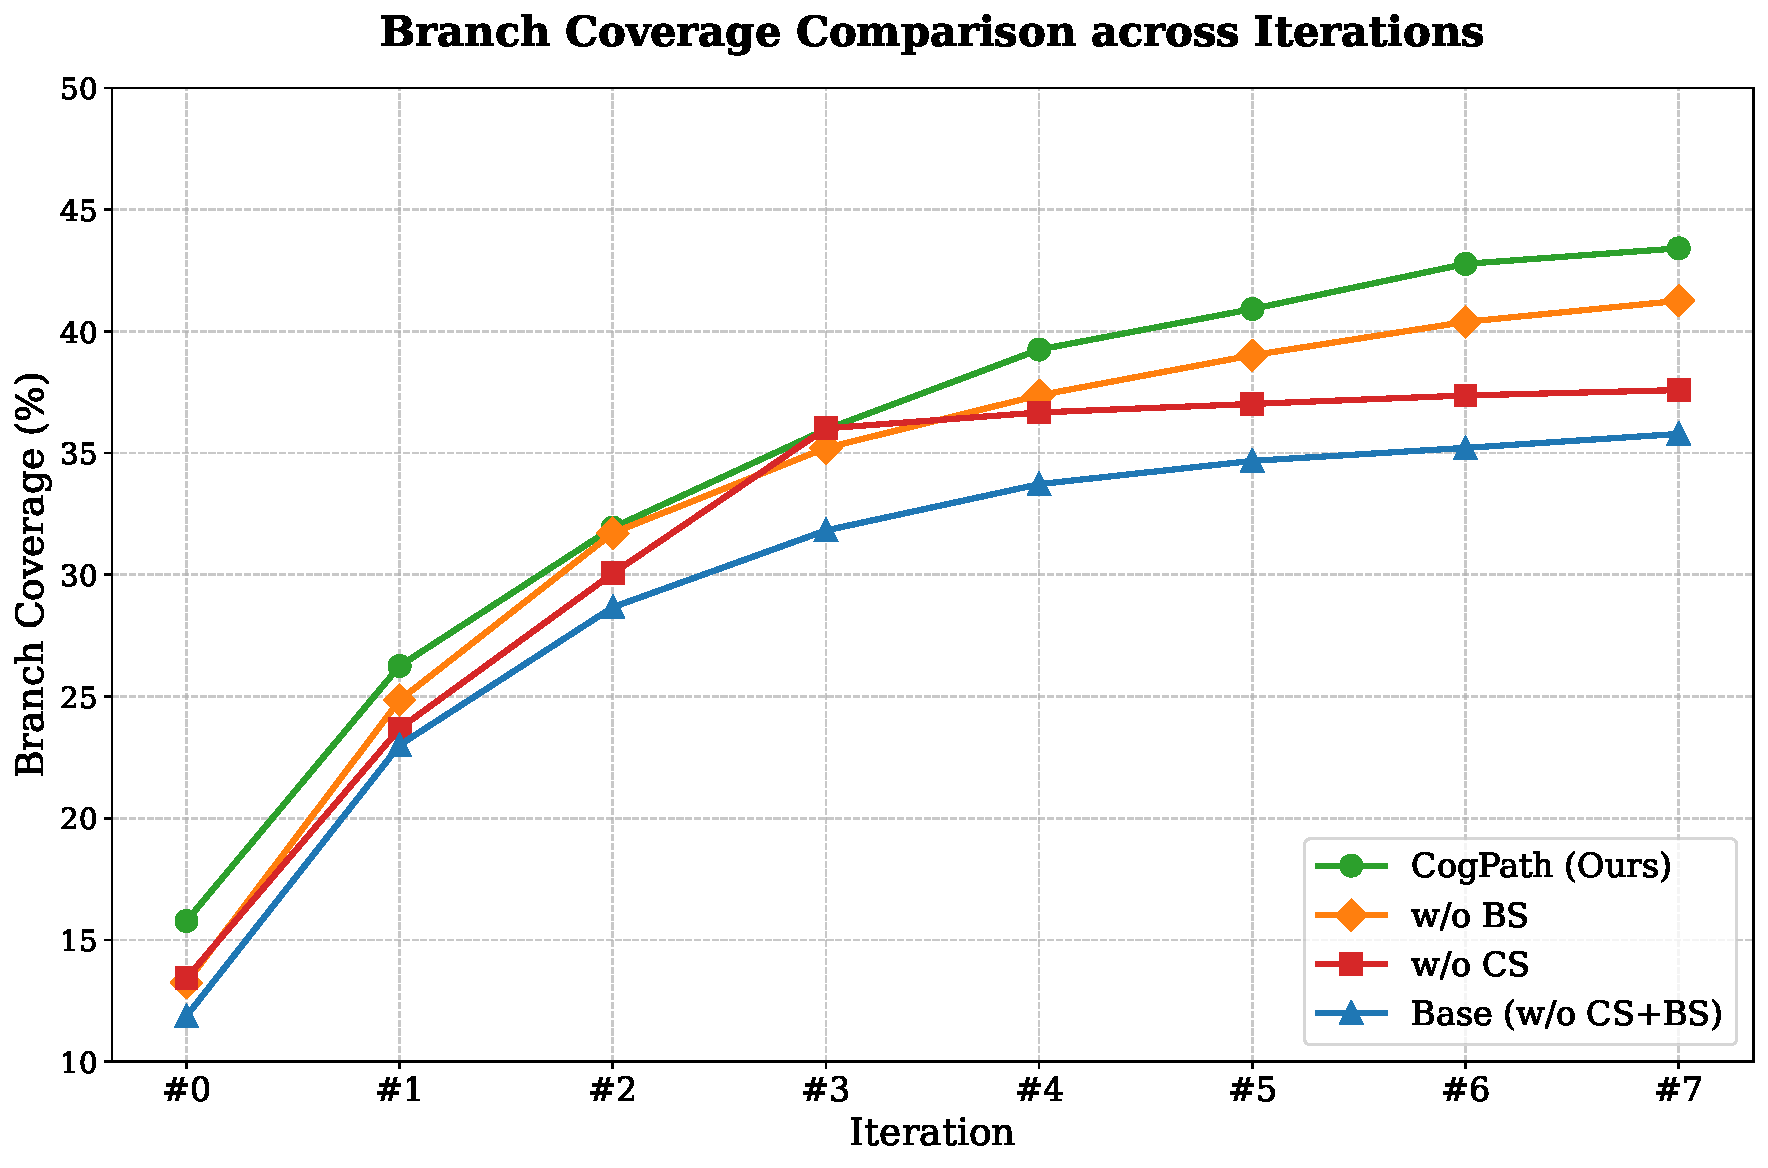
\includegraphics[width=\linewidth]{figures/branch_coverage_comparison.pdf}
    \caption{Branch coverage improvement over iterations for \ourmethod{} and its three ablated variants.}
    \label{fig:branch-growth}
\end{figure}

Figure~\ref{fig:branch-growth} traces branch coverage across iterations for all four configurations. \ourmethod{} consistently achieves the highest coverage at every iteration and exhibits the steepest growth curve, demonstrating that both BS and CS contribute not only to final coverage but also to the efficiency of iterative improvement. In contrast, removing either component leads to slower convergence, and removing both produces the flattest growth trajectory, underscoring the necessity of each component for sustained progress.

\begin{tcolorbox}[colback=gray!5, colframe=gray!100, title=Answer to RQ2]
Both BS and CS make independent and complementary contributions to \ourmethod{}. BS provides the larger share of improvement by eliminating irrelevant context ($-$5.94 pp when removed), while CS explicitly guides the LLM toward satisfying cross-method preconditions ($-$4.62 pp when removed). Removing both components degrades BC by 7.84 pp on average, with per-project drops reaching up to 27.49 pp (\textit{Csv}), confirming that neither component is redundant. The iterative growth curves further show that both components contribute to the efficiency of coverage accumulation across generation rounds.
\end{tcolorbox}

\subsection{RQ3: Performance Comparison of Different LLMs}
\begin{table*}[t]
\centering
\caption{Model Generalization Across Different LLMs}
\label{tab:model-generalization}
\small
\begin{tabular}{@{} l c c c c c c c c c c @{}}
\toprule
\multirow{2}{*}{Project} & \multirow{2}{*}{\#C} & \multirow{2}{*}{CC} &
\multicolumn{2}{c}{QC3-30B} & \multicolumn{2}{c}{GPT-5.4-Mini} & \multicolumn{2}{c}{QW3.5-397B} & \multicolumn{2}{c}{DS-V3.1} \\
\cmidrule(lr){4-5} \cmidrule(lr){6-7} \cmidrule(lr){8-9} \cmidrule(lr){10-11}
& & & LC(\%) & BC(\%) & LC(\%) & BC(\%) & LC(\%) & BC(\%) & LC(\%) & BC(\%) \\
\midrule
Cli & 2 & 11.00 & 84.32 & 70.73 & 97.86 & 86.18 & 98.82 & 92.63 & 98.82 & 91.93 \\
Codec & 7 & 16.14 & 76.97 & 69.60 & 89.78 & 82.61 & 98.32 & 95.30 & 93.60 & 88.46 \\
Collections & 5 & 18.60 & 40.46 & 34.63 & 98.31 & 94.14 & 98.16 & 94.43 & 98.02 & 94.20 \\
Compress & 9 & 15.33 & 36.09 & 29.05 & 87.15 & 80.29 & 86.92 & 80.90 & 81.32 & 76.04 \\
Csv & 3 & 16.67 & 62.27 & 52.29 & 87.42 & 77.76 & 95.71 & 87.42 & 85.70 & 77.53 \\
Gson & 4 & 23.25 & 63.82 & 41.24 & 90.26 & 83.06 & 92.88 & 87.97 & 92.13 & 82.86 \\
JCore & 9 & 16.33 & 41.72 & 35.54 & 63.71 & 57.83 & 83.25 & 76.77 & 66.62 & 57.76 \\
JDatabind & 9 & 15.33 & 23.35 & 17.85 & 76.16 & 68.78 & 74.93 & 69.81 & 84.06 & 77.44 \\
JXml & 4 & 21.50 & 20.61 & 17.08 & 73.41 & 74.20 & 62.20 & 63.65 & 66.06 & 65.22 \\
Jsoup & 8 & 14.13 & 66.43 & 52.55 & 93.37 & 82.96 & 95.87 & 87.49 & 87.15 & 79.98 \\
JxPath & 12 & 15.50 & 42.28 & 35.84 & 81.72 & 75.11 & 71.30 & 66.22 & 76.89 & 73.21 \\
Lang & 17 & 16.88 & 59.21 & 52.14 & 90.65 & 84.32 & 91.72 & 87.44 & 88.21 & 85.02 \\
Math & 30 & 16.47 & 59.60 & 54.02 & 88.89 & 81.82 & 92.96 & 87.47 & 91.69 & 85.41 \\
Time & 11 & 17.36 & 66.79 & 59.25 & 94.18 & 87.63 & 96.94 & 91.08 & 94.71 & 89.92 \\
\midrule
\multicolumn{3}{l}{Average} & 53.14 & 44.41 & 86.63 & 79.76 & 88.57 & 83.47 & 86.07 & 80.36 \\
\bottomrule
\end{tabular}
\end{table*}


Table~\ref{tab:model-generalization} reports LC and BC achieved by \ourmethod{} under four LLMs across all 14 projects. We discuss the results from three perspectives.

\noindent\textbf{Overall generalizability.}\ourmethod{} delivers consistently strong performance regardless of the underlying LLM, confirming that its coverage gains derive from the structural guidance of BS and CS rather than from any model-specific behavior.The three large-scale models—GPT-5.4-Mini, QW3.5-397B, and DS-V3.1—achieve average BC of 79.76\%, 83.47\%, and 80.36\%, respectively, whereas QC3-30B reaches 44.41\%.Despite this gap, QC3-30B already outperforms all baselines in RQ1 (best competitor: HITS at 34.24\%), demonstrating that \ourmethod{}'s framework-level contributions are effective even under limited model capacity.

\noindent\textbf{Interaction between model capacity and cyclomatic complexity.}The performance gap between QC3-30B and large models is not uniform across projects but is strongly modulated by cyclomatic complexity and inter-method dependency depth.On \texttt{Collections} (CC$_{avg}$ = 18.60), QC3-30B achieves only 34.63\% BC, while all three large models reach $\sim$94\%, a gap of nearly 60 pp.Similarly, on \texttt{Gson} (CC$_{avg}$ = 23.25, the highest in the benchmark), the gap exceeds 40 pp.In contrast, on lower-complexity projects such as \texttt{Cli} and \texttt{Time}, the gap narrows to under 20 pp, suggesting that \ourmethod{}'s structural guidance can partially compensate for limited model capacity when branch conditions are relatively straightforward.This pattern indicates that the primary bottleneck for QC3-30B is not the framework structure but the model's inability to perform the multi-step object initialization required by complex preconditions—precisely the reasoning that Constraint-Hints is designed to elicit.

\noindent\textbf{Synergy between Constraint-Hints and model reasoning capacity.}Cross-referencing with the ablation results in RQ2, CS contributes most on projects with deep cross-method dependencies (e.g., \texttt{JDatabind}: $-$8.52 pp when removed).These are also the projects where the capacity gap between QC3-30B and large models is most pronounced.This co-occurrence suggests a synergistic relationship: Constraint-Hints provides the LLM with explicit preconditions, but fully exploiting these hints requires multi-step reasoning capabilities that only sufficiently large models possess.In other words, CS lowers the reasoning barrier, while larger models are better positioned to clear it.

\noindent\textbf{Residual challenges across all models.}Despite the strong overall performance of large models, certain projects remain challenging regardless of model capacity.On \texttt{JCore} and \texttt{JXml}, the best-achieved BC across all large models stays below 77\% and 75\%, respectively.Manual inspection indicates that these projects contain deeply nested control flows where backward slicing occasionally produces overly coarse slices, inadvertently removing type information required for mock construction—a limitation identified in RQ2 that persists under stronger models.Furthermore, project-level variation among large models exists: on \texttt{JXml}, GPT-5.4-Mini (74.20\%) outperforms QW3.5-397B (63.65\%), while on \texttt{JCore}, DS-V3.1 (57.76\%) falls behind QW3.5-397B (76.77\%).Such sensitivity likely reflects model-specific differences in handling ambiguous or incomplete type hierarchies, which represents an avenue for future investigation.

\begin{tcolorbox}[colback=gray!5,colframe=gray!100, title=Answer to RQ3]
\ourmethod{} generalizes robustly across LLMs of varying scales and architectures.Model capacity plays a critical role: large-scale models outperform QC3-30B by up to 59.5 pp in BC, with the gap most pronounced on high-complexity projects requiring multi-step reasoning—precisely where Constraint-Hints provides the most structural guidance.Nonetheless, even QC3-30B surpasses all baselines in RQ1, confirming that \ourmethod{}'s framework-level design contributes independently of model capacity.Among large models, performance is broadly comparable, though residual challenges on projects with coarse-grained slicing sensitivity point to opportunities for further refinement.
\end{tcolorbox}